\documentclass{article}
\usepackage{graphicx}
\usepackage{varwidth}
%\usepackage{caption}
\begin{document}
%	this is dog picture
%	\begin{figure}
%		
\includegraphics[scale=0.4]{snuggle.jpg}
%		\caption{in plain format, if title too long, like normal paragraphics for display. 
%		if you set the formal small title,you can cut for paragraphics}
%	\end{figure}\par
%	this is cat type table
%	\begin{table}
%		\begin{tabular}{c|c|c}
%			name & sex & grade\\
%			\hline
%			lily & female & 6\\
%			lucy & female & 4\\
%			peter & male & 6\\
%		\end{tabular}
%		\caption{student information}
%	\end{table}\par
	\begin{figure}
		\centering
		\begin{varwidth}[t]{\textwidth}
			\vspace{0pt}
			
\includegraphics[scale=0.2]{snuggle.jpg}
		\end{varwidth}
		\begin{varwidth}[t]{\textwidth}
			\vspace{0pt}
			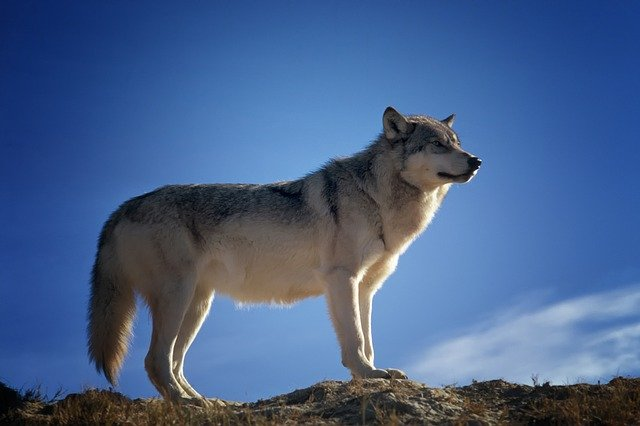
\includegraphics[scale=0.2]{wolf.jpg}
		\end{varwidth}
	\end{figure}
\end{document}


% begin{figure}...\end{figure}用于图片浮动体

% begin{table}...\end{table}用于表格浮动体

% 共同可选参数列表:
% h - 浮动体根据上下文顺序排列
% t - 浮动体排在当前页或下一页页首
% b - 浮动体排在当前页页尾
% p - 浮动体另外一页进行排列
% 参数的优先级与顺序无关,通常按htbp顺序排列;当只有h参数时,拓展为ht参数集合;默认参数集合为tbp

% LaTeX最多同时保存18个未处理的浮动体

% \caption{string}为浮动体中的标题

% 在同一个浮动体中,表格和图标盒子可以并列排放。其中,表格按垂直方向居中对其,图片按垂直方向的基准线对齐

% \begin{varwidth}[t]{\textwidth}...\end{varwidth}用于确定宽度,\vspace{0pt}用于配置一个0pt空行,并按空行进行对齐
 